\section{Case Study and Experiments} \label{sec:casestudy}
In this section, we will study the use of the proposed on-accelerator training framework 
on three typical scenarios including CNN accelerator with approximate multiplier, 
CNN accelerator with overclocking and CNN accelerator with soft errors, 
in which the CNN accelerator produces undetermined computing result of neural networks.
Each application scenario is analyzed with comprehensive experiments. 
Finally, we further present some general on-accelerator training experiment to 
exhibit the training time and optimization.

For scenarios of approximate computing and overclocking, we experimented on the 8-bit 
fixed-point PipeCNN \cite{pipecnn_2} on Xilinx KCU1500 board. For the case of soft error, 
we analyzed with an equivalent C model of PipeCNN due to the lack of 
HLS based soft error injection tools. To evaluate the training, 
we take four representative convolution neural networks including LeNet, 
AlexNet, VGG-16 and VGG-19 as the benchmark in the experiments. The neural network 
benchmark is summarized in Table \ref{tab:CNN-table}. It covers networks with 
diverse sizes and the analysis can be applied to more neural networks.

\begin{table}
        \centering
        \vspace{-0.3em}
        \caption{Neural network benchmark}
        \label{tab:CNN-table}
        \vspace{-0.3em}
        \begin{tabular}{c|c|c|c}
		\toprule
		  & Dataset & Layers & Total weights \\
		\midrule
		LeNet & Mnist & 4 & 60K \\
		\midrule
		AlexNet & ImageNet & 8 & 61M \\
		\midrule
		VGG-16 & ImageNet & 16 & 138M \\
		\midrule
		VGG-19 & ImageNet & 19 & 143M \\
		\bottomrule
        \end{tabular}
        \vspace{-1em}
\end{table}


\subsection{CNN accelerator with approximate arithmetic logic}
Approximate arithmetic logic that promises high-performance and energy-efficient computing has 
been studied intensively in prior work. When the approximate arithmetic logic 
is used in a CNN accelerator, the computing result of a neural network will be different 
from the exact computing result and lead to prediction accuracy loss when deploying 
the neural network model directly as shown in Section \ref{sec:motivation}. 
An intuitive approach is to train with software simulation, but some of the approximate arithmetic 
operators are rather complex when simulated with software. Particularly, some of the 
approximate arithmetic unit relies on underlying semiconductor devices which 
can hardly be simulated with software. In this cases, the proposed on-accelerator 
training framework fits well with this situation. 

In this experiment, we mainly focus on the prediction accuracy loss and 
take the dynamic-range approximate multiplier proposed in \cite{Approximate_Multiplier_31} as 
an approximate computing example. The multiplier is implemented on top of the PipeCNN
accelerator. Basically, it reserves the most significant non-zero bits as well as the 
following $k$ lower bits. Larger $k$ will keep more valid digits and the multiplier 
is more accurate. On the contrast, smaller $k$ leads to lower precision but 
more efficient computing. 

Figure \ref{fig:k2-approximate-multiplier} shows the 
neural network prediction accuracy when running on the approximate CNN 
accelerator with $k=2$. According to the accuracy comparison of the models with 
offline training and on-accelerator training, it can be find that the 
top1 and top5 prediction accuracy improvement is up to xx and xx respectively. 
When $k=3$, the offline trained model accuracy is much higher due to the improved 
computing precision leaving little optimization space. The average prediction 
accuracy is still improved, though the improvement is less significant.
\begin{figure}
        \center
        \subfloat[top1]{
                \label{fig:appro-k2-top1}
                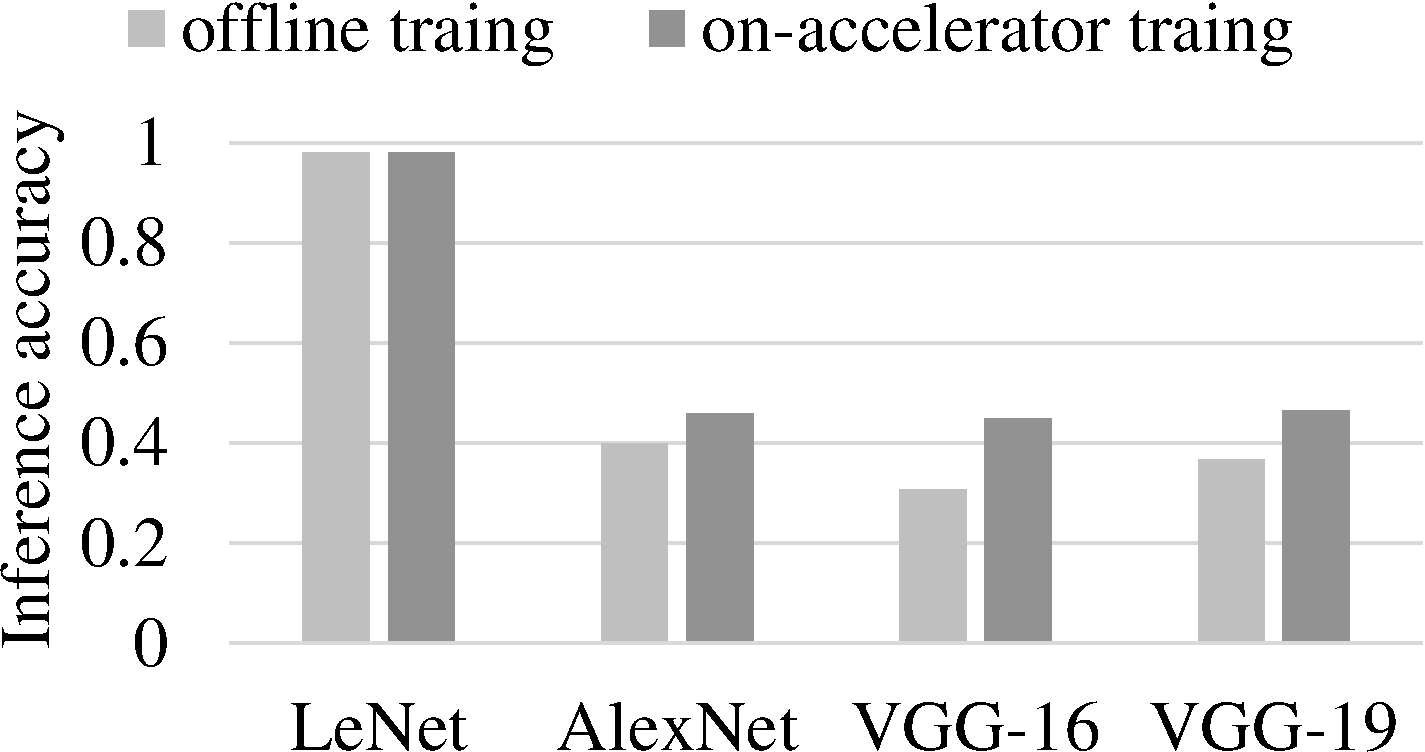
\includegraphics[width=0.65\linewidth]{appro-k2-top1}
        }
        \qquad
        \subfloat[top5]{
                \label{fig:appro-k2-top5}
                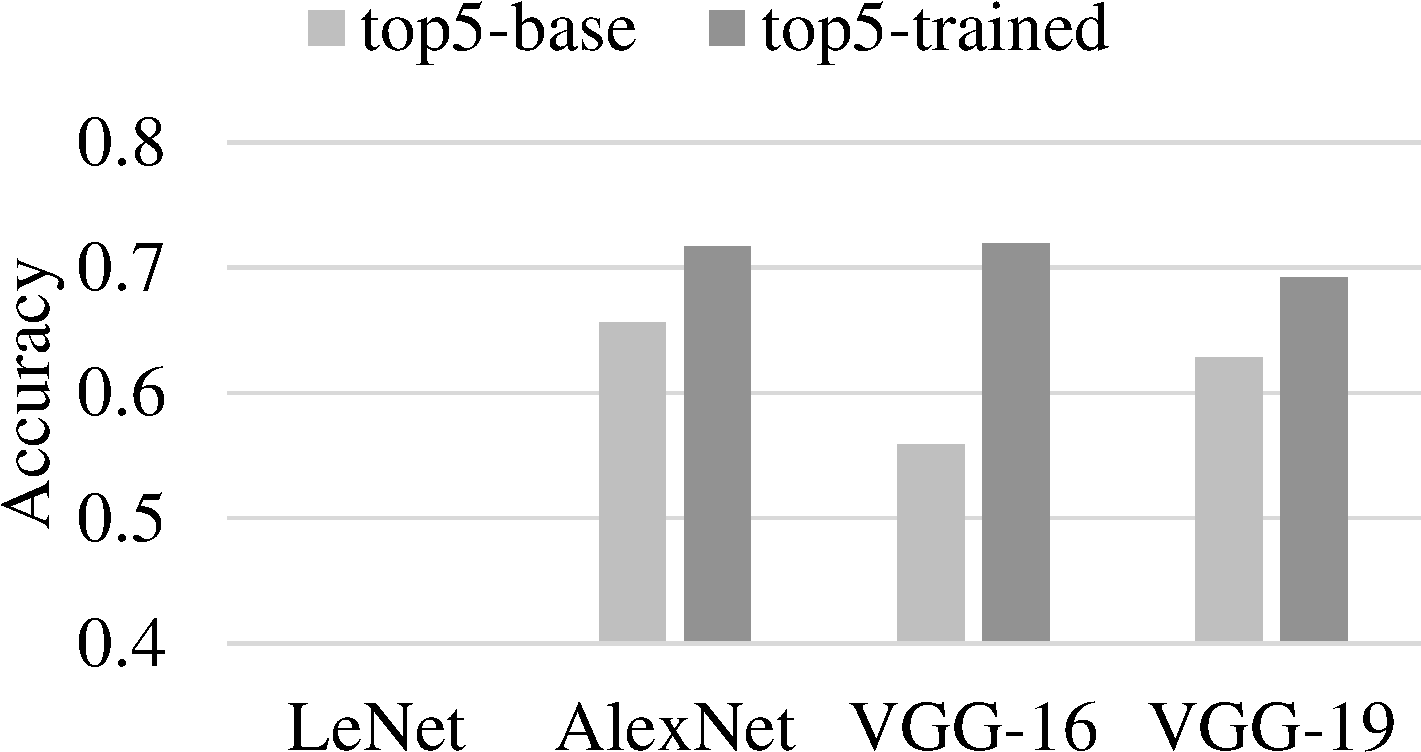
\includegraphics[width=0.65\linewidth]{appro-k2-top5}
        }
        \caption{The prediction accuracy of the neural network on accelerator with approximate multiplier(k=2)}
        \label{fig:k2-approximate-multiplier}
\end{figure}

\begin{figure}
        \center
        \subfloat[top1]{
                \label{fig:appro-k3-top1}
                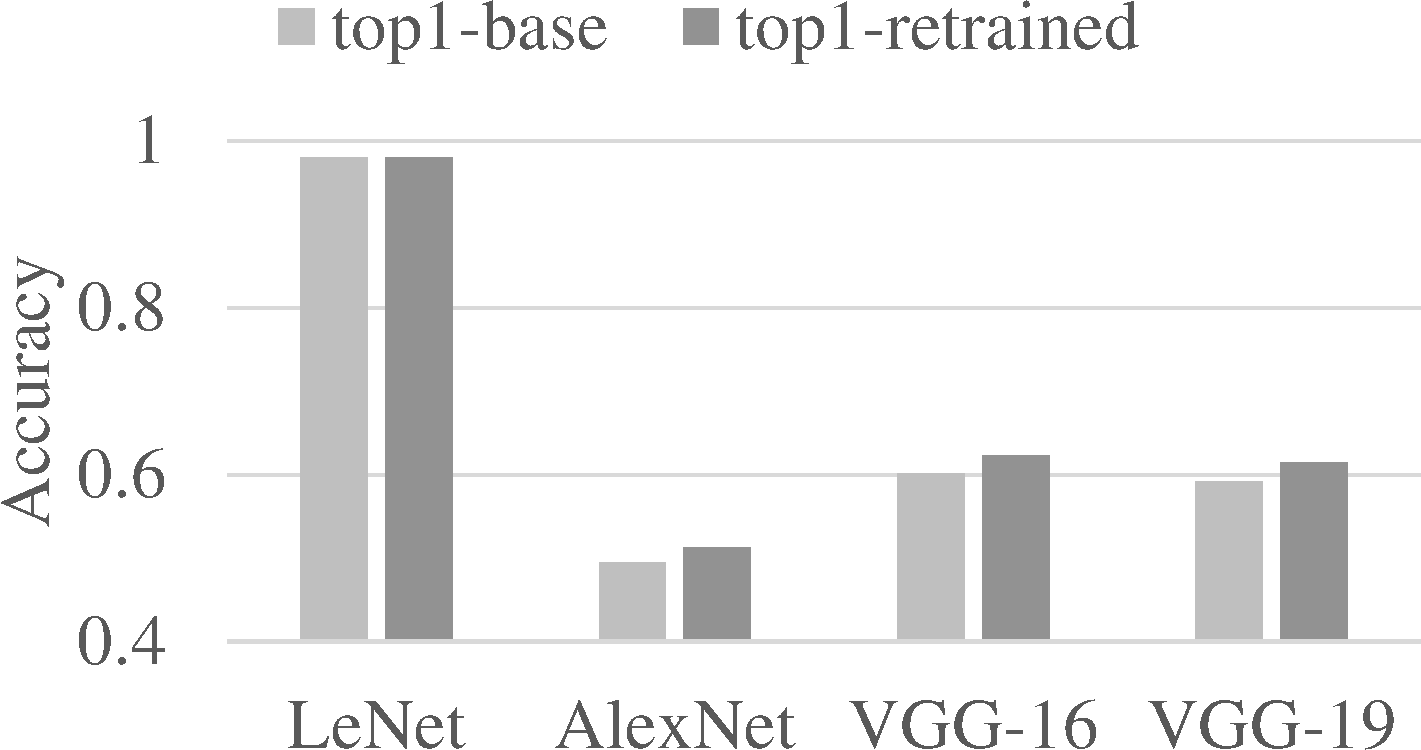
\includegraphics[width=0.6\linewidth]{appro-k3-top1}
        }
        \qquad
        \subfloat[top5]{
                \label{fig:appro-k3-top5}
                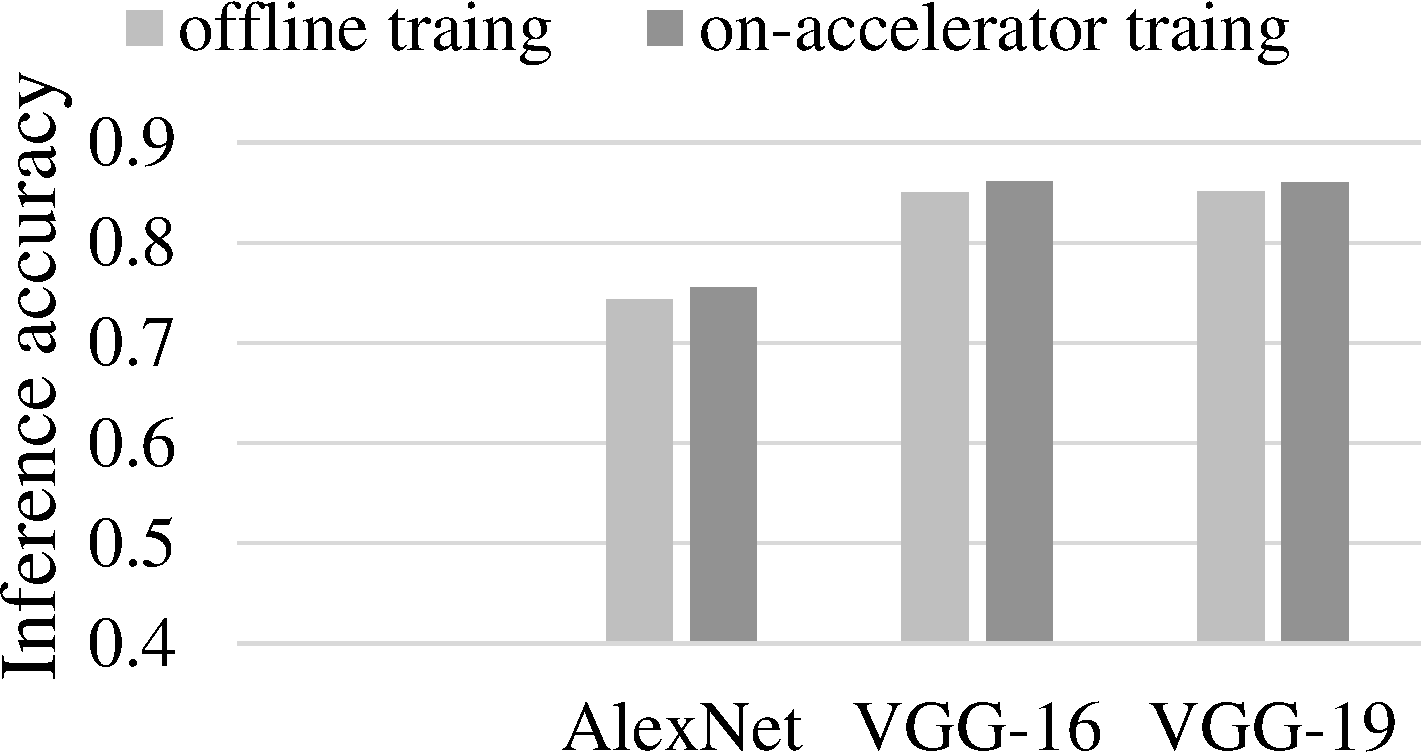
\includegraphics[width=0.6\linewidth]{appro-k3-top5}
        }
        \caption{The Accuracy of Four CNN models on accelerators with approximate multiplier(k=3)}
        \label{fig:k3-approximate-mltiplier}
\end{figure}

\subsection{CNN accelerator with overclocking}
Clock frequency is almost proportional to the performance of the CNN accelerator 
especially for large convolution operation which is typically computing bound. 
However, the circuit design tools typically adopt conservative design options 
in order to avoid the timing violations in the worst case. Overclocking enables 
higher clock frequency and performance, but timing errors may happen and affect 
the inference accuracy. In this case, we can also apply the on-accelerator 
training to have the computing errors tolerated by the models without 
redesigning the CNN accelerator.

With PipeCNN, we implemented the benchmark neural networks on Xilinx KCU1500. 
LeNet and AlexNet use the same hardware implementation 
while VGG-16 and VGG-19 share the same hardware implementation. 
The two implementations work at 210 MHz and 190 MHz respectively.
With overclocking, they can be boosted to 210 MHz - 260 MHz and 
190 MHz - 240 MHz respectively. Given different overclocking frequency, 
the accelerator produces different computing results due to the variable
timing errors. It is expected that more aggressive overclocking incur 
more computing errors and precision loss. To gain both the higher clock 
frequency and less prediction loss, we can also adopt the proposed on-accelerator 
training framework for overclocked CNN accelerator. 

The prediction accuracy comparison on different overclocking is presented in Figure \ref{fig:overclock-accuracy}. 
It shows that the overclocking can enhance the clock frequency by 19\% to 26\%. 
While applying the off-line trained model 
to the accelerator with overclocking, the top-5 accuracy degrades by up to 4.3\%. When the proposed training 
framework is used, the resulting retrained model can be much better especially near the overclocking limit.

  For AlexNet, VGG-16 and VGG-19, the top-5 accuracy of the retained models is improved by 3.4\%, 1.8\%, and 2\% 
respectively at the extreme overclocking frequency. For LeNet which is a rather small yet reliable network 
compared to the other three, the implementation remains unaffected even when the clock is boosted to 260 MHz 
from 210 MHz. When the clock goes up to 270MHz, the timing error can no longer be tolerated by the hardware system, 
the prediction accuracy drops to 10\% which is essentially meaningless. In this case, the base model 
and the retrained model is pretty much the same. To ensure the stability of the overclocking experiment, 
we also keep measuring the accuracy of the accelerators with extreme overclocking. With repeatedly 
running the test for up to 40 hours, the measured accuracy varies slightly as present in Figure 7. 
Despite the fact that the errors caused by the overclocking can be hardly modeled precisely at runtime, 
the inherent error patterns may still partly be captured by the CNN model with the proposed training. 
This explains the higher prediction accuracy with the retrained model. According to the 
above experiments, we can conclude that the proposed accelerator aware training can produce 
more resilient CNN model tolerating errors caused by intensive overclocking. 

\begin{figure}
        \center
	\subfloat[LeNet]{
		\label{fig:lenet}
		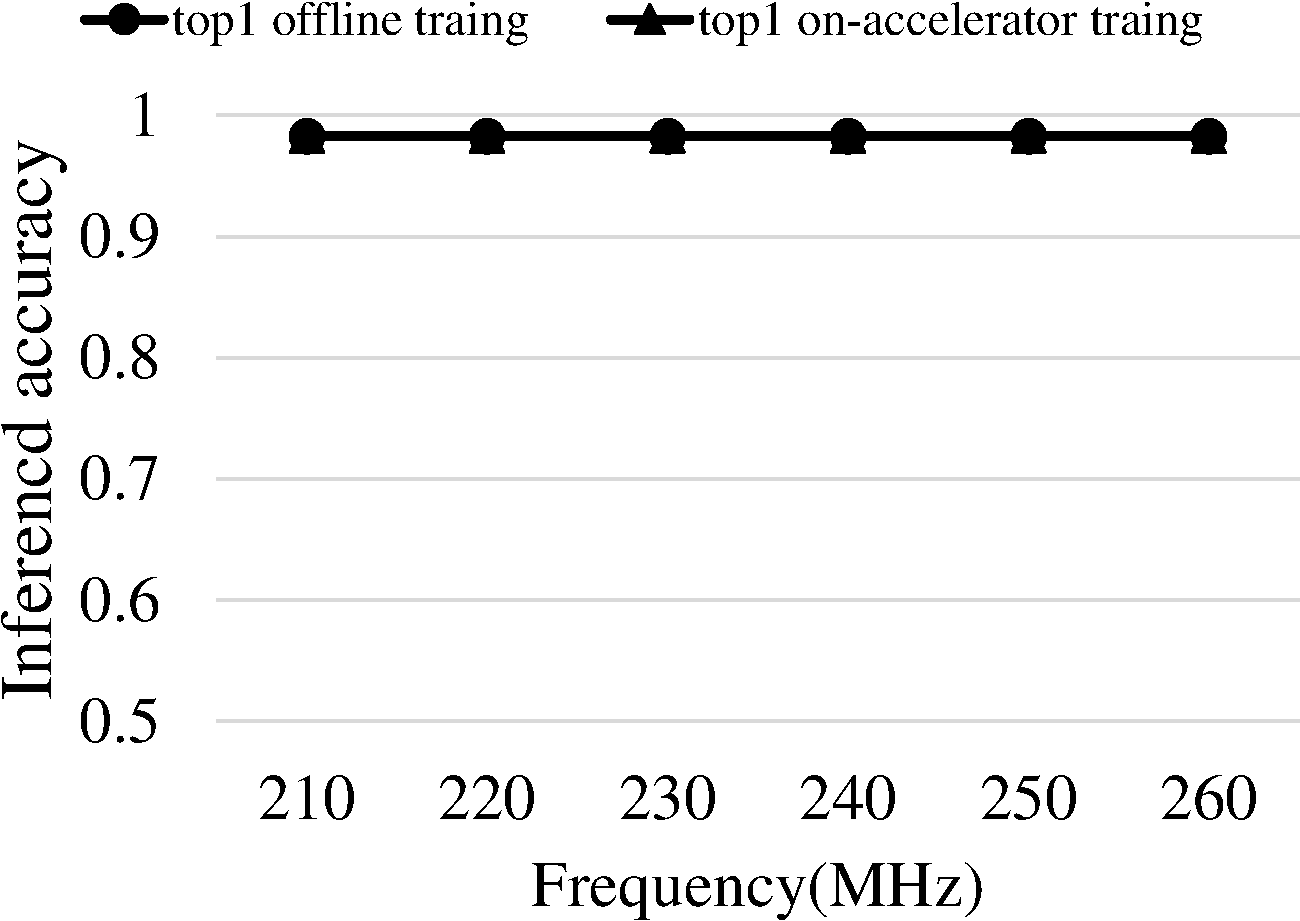
\includegraphics[width=0.6\linewidth]{lenet-overclock}
	}
	\qquad
	\subfloat[AlexNet]{
                \label{fig:alexnet}
                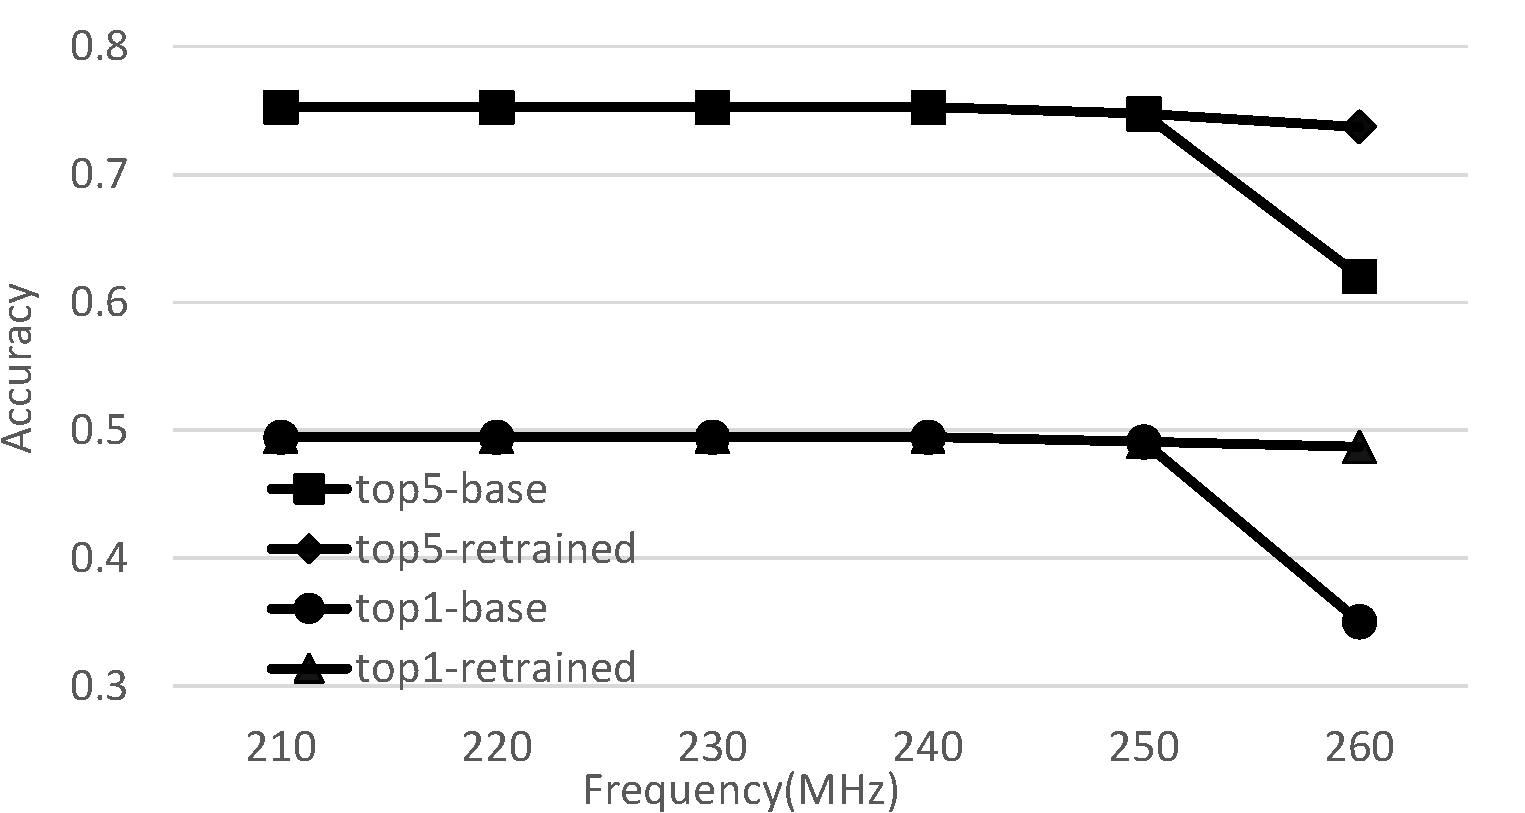
\includegraphics[width=0.6\linewidth]{alexnet-overclock}
        }
	\qquad
	\subfloat[VGG-16]{
                \label{fig:vgg16}
                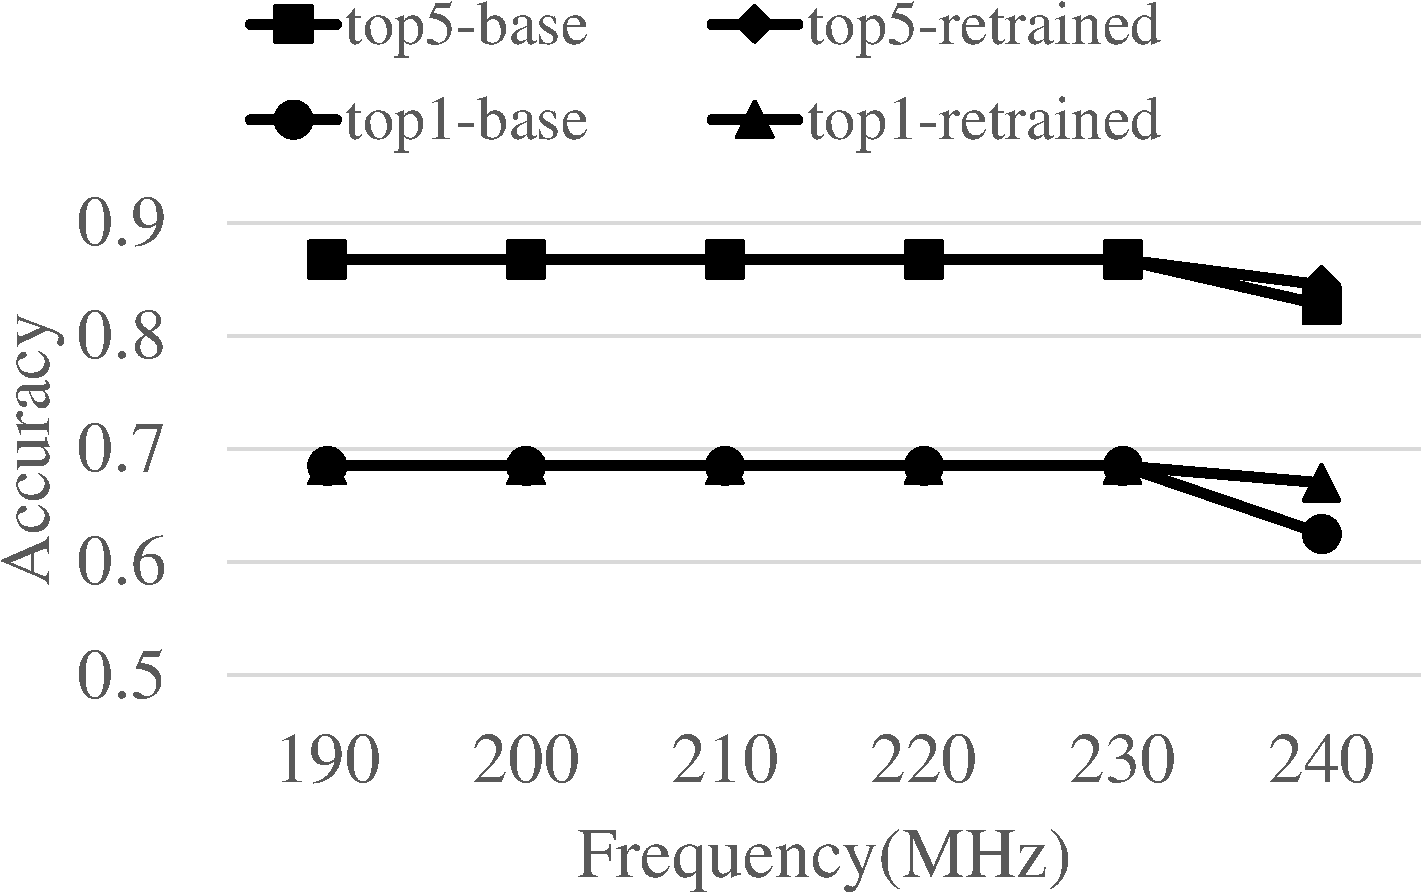
\includegraphics[width=0.6\linewidth]{vgg16-overclock}
        }
        \qquad
	\subfloat[VGG-19]{
                \label{fig:vgg19}
                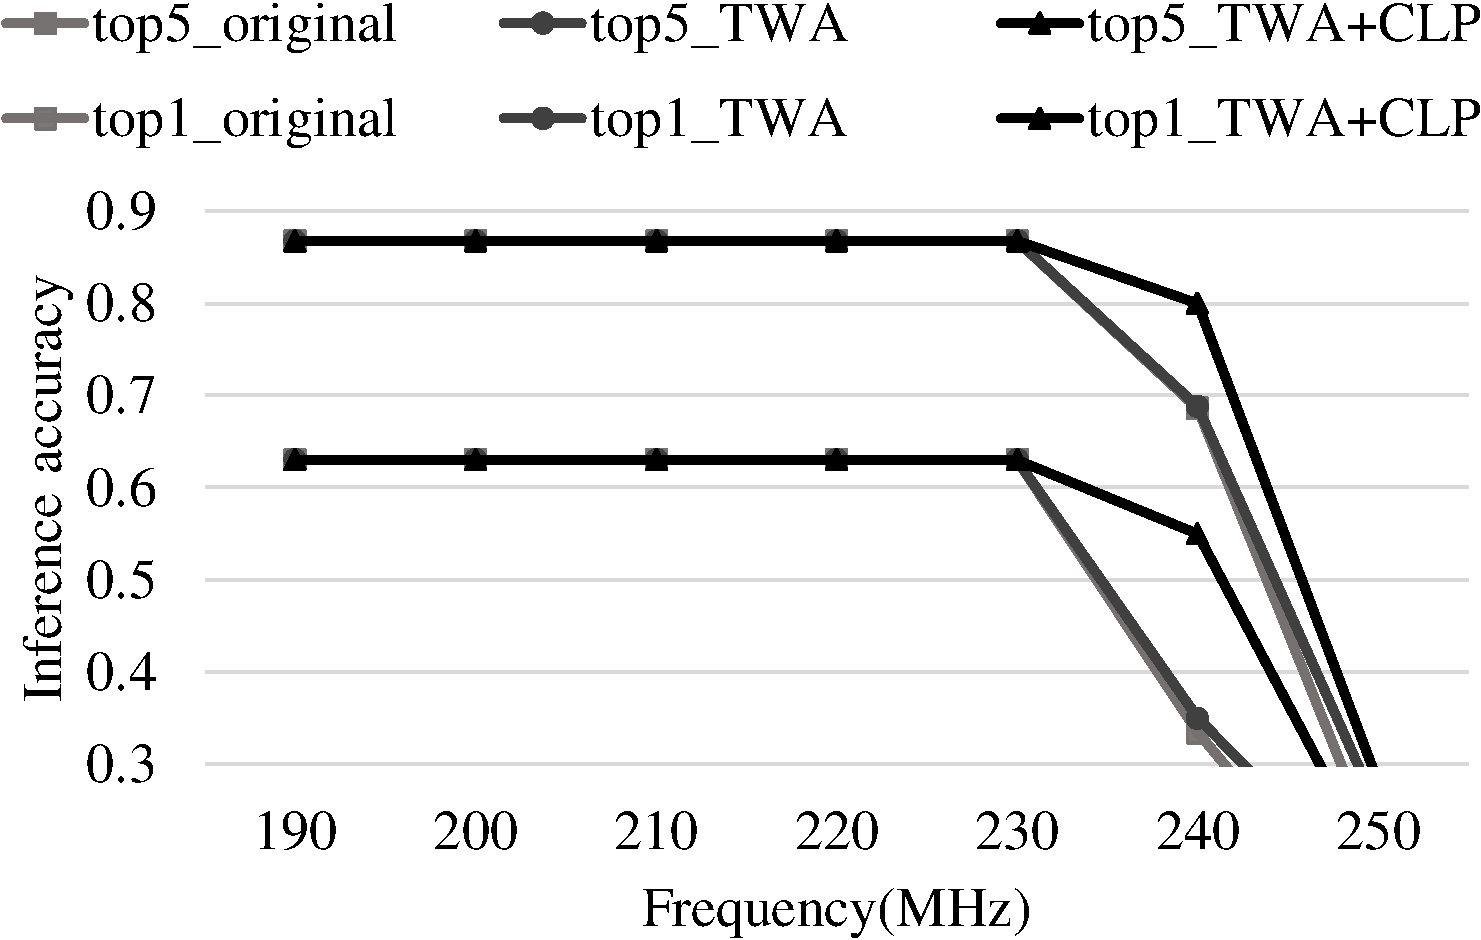
\includegraphics[width=0.6\linewidth]{vgg19-overclock}
        }
	\caption{The prediction accuracy of the benchmark neural networks on accelerators with different overclocking}
        \label{fig:overclock-accuracy}
\end{figure}

To ensure the stability of the overclocking experiment, we 
also keep measuring the accuracy of the accelerators with extreme 
overclocking. With repeatedly running the test for up to 40 hours, 
the measured accuracy varies slightly as present in Figure 7. 
Despite the fact that the errors caused by the overclocking can be 
hardly modeled precisely at runtime, the inherent error patterns may 
still partly be captured by the CNN model with the proposed training. 
This explains the higher prediction accuracy with the retrained model. 
According to the above experiments, we can conclude that the proposed 
accelerator aware training can produce more resilient CNN model tolerating 
errors caused by intensive overclocking. 

\begin{figure}
        \center{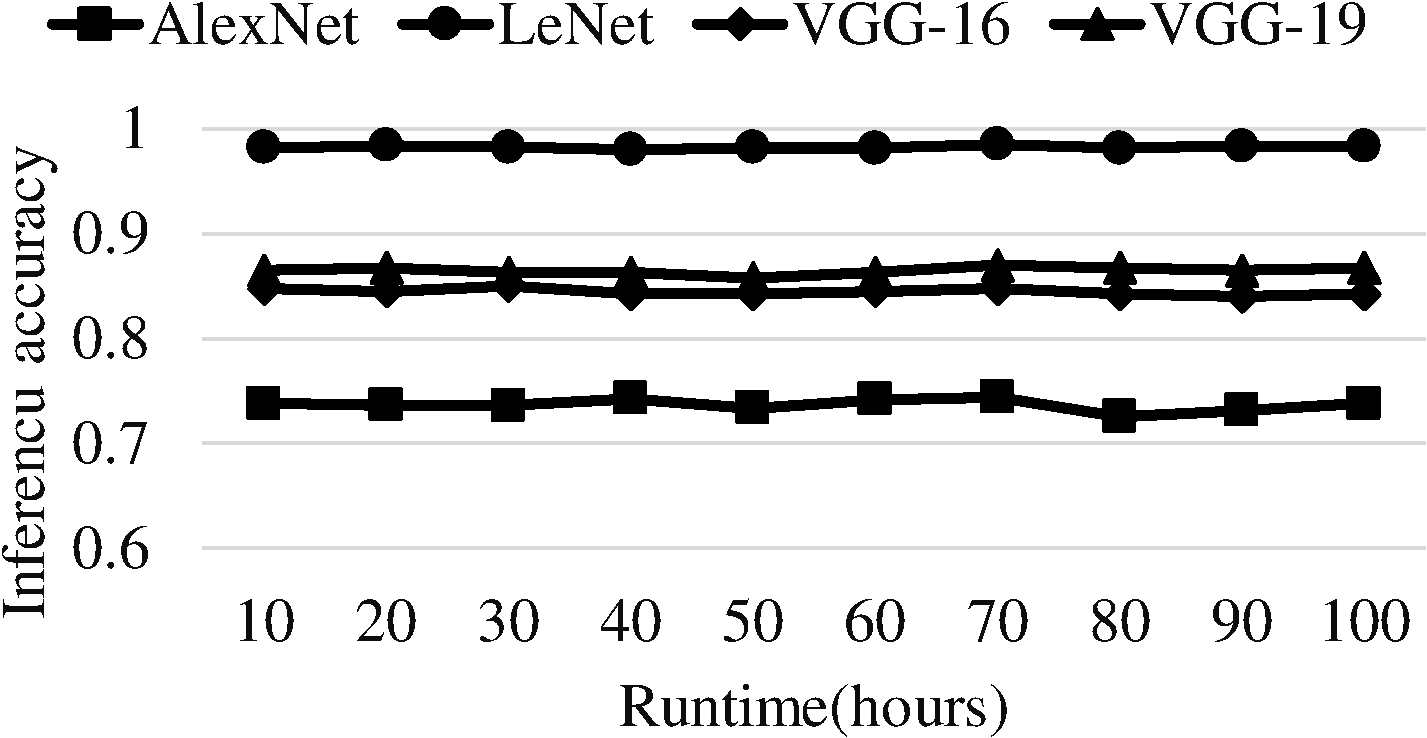
\includegraphics[width=0.6\linewidth]{stability}}
        \caption{The Stability of Retrained Model}
        \label{fig:stability}
%        \vspace{-0.5em}
\end{figure}

  Finally, we also present the training time on the hybrid CPUFPGA architecture. 
It can be seen that the training is much slower than the fixed-point training on CPU. 
This is mainly caused by the frequently data transferring between device memory and host 
memory in the proposed training, while this will not affect the inference time. In addition, 
we can also find that the training on larger network takes longer time and higher clock frequency 
is also beneficial to the training time as expected. 

\begin{figure}
        \center{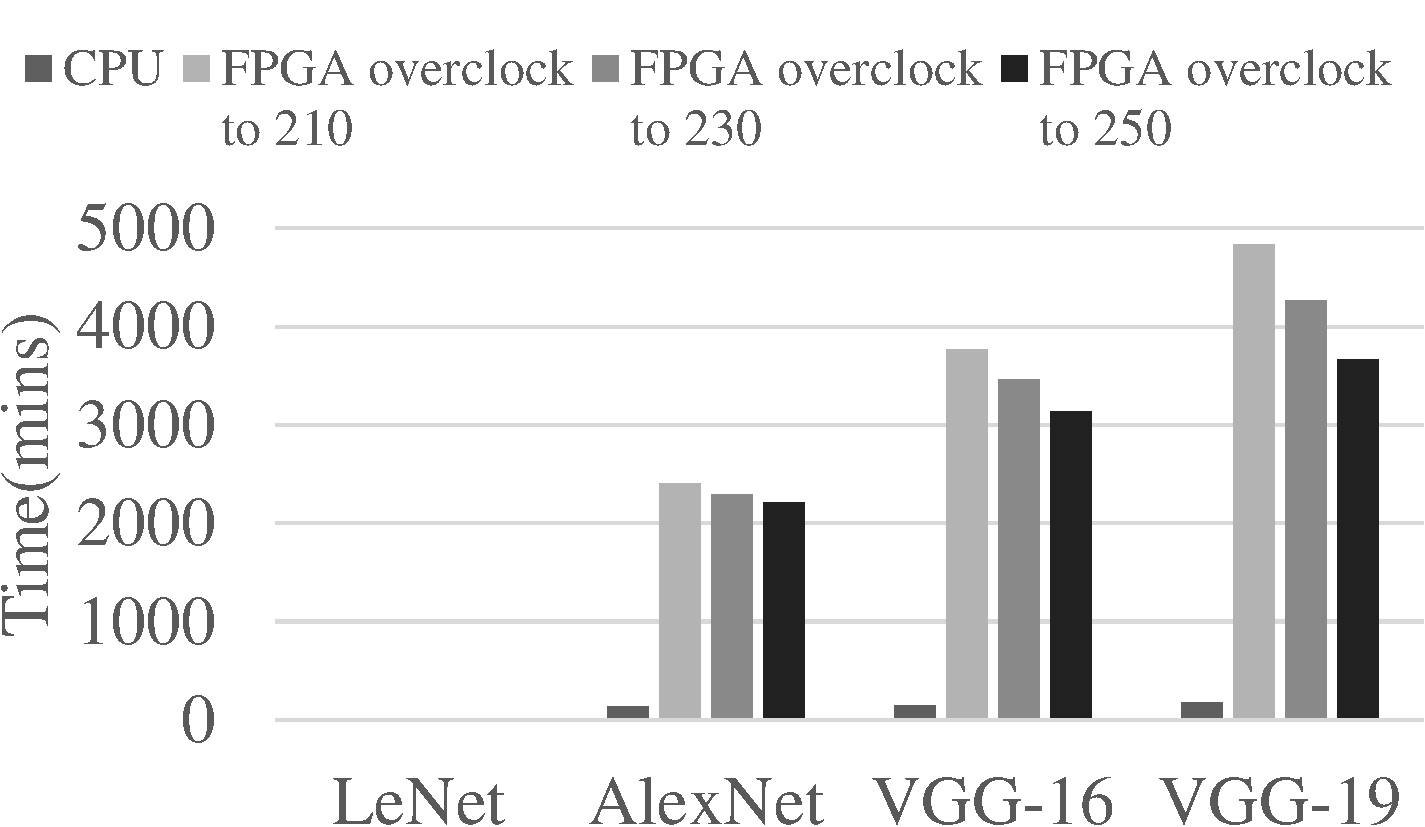
\includegraphics[width=0.6\linewidth]{time}}
        \caption{Training time}
        \label{fig:time}
%        \vspace{-0.5em}
\end{figure}

\subsection{CNN accelerator with soft errors}
  With the shrinking semiconductor feature size and increasing FPGA capacity, 
FPGA design gets error-prone to the transient faults (often known as soft errors). 
They can affect the behaviors of the FPGA design dramatically. Many researchers \cite{Mansour_20,Karim_21,Nidhin_22,Subasi_23,ROSCH_24} 
have proposed diverse approaches to address this problem. While CNN accelerators on FPGA can be different 
from general hardware design because the CNN model deployed can be further trained and tolerate the 
soft errors as proposed in prior section\cite{Tu2018RANA_1}.

  To explore the influence of soft errors on CNN accelerator, we need to inject soft errors to the system first. 
A number of fault injection techniques have been proposed in prior literature. In this work, we adopt 
a simple software simulation- based method to inject random errors. Although the error may be caused by 
on-chip memory or other SRAM cells, we have a random bit of the computing result flipped at a specific rate. 
The simple yet representative model will not increase the training time too much.

  We also take LeNet, AlexNet, VGG-16, and VGG-19 to evaluate the influence of soft errors on prediction accuracy,
the top-5 accuracy of the resulting implementations is presented in Figure 9. When we gradually 
increase the error rate from 1E-7 to 1E-5, the prediction accuracy degrades accordingly when applying the off-line 
trained model directly on the faulty accelerator. When the error rate goes up to 1E-4.5, 
the accuracy in the worst case drops by around 13.5\%. Similar to overclocking, LeNet can tolerate 
more errors than the other three networks. The accuracy remains unchanged until the error rate reaches 1E-3. 
When the error injection rate is low, the CNN model is able to cover almost all the negative influence 
on the prediction accuracy.

\begin{figure}
        \center
        \subfloat[LeNet]{
                \label{fig:lenet}
                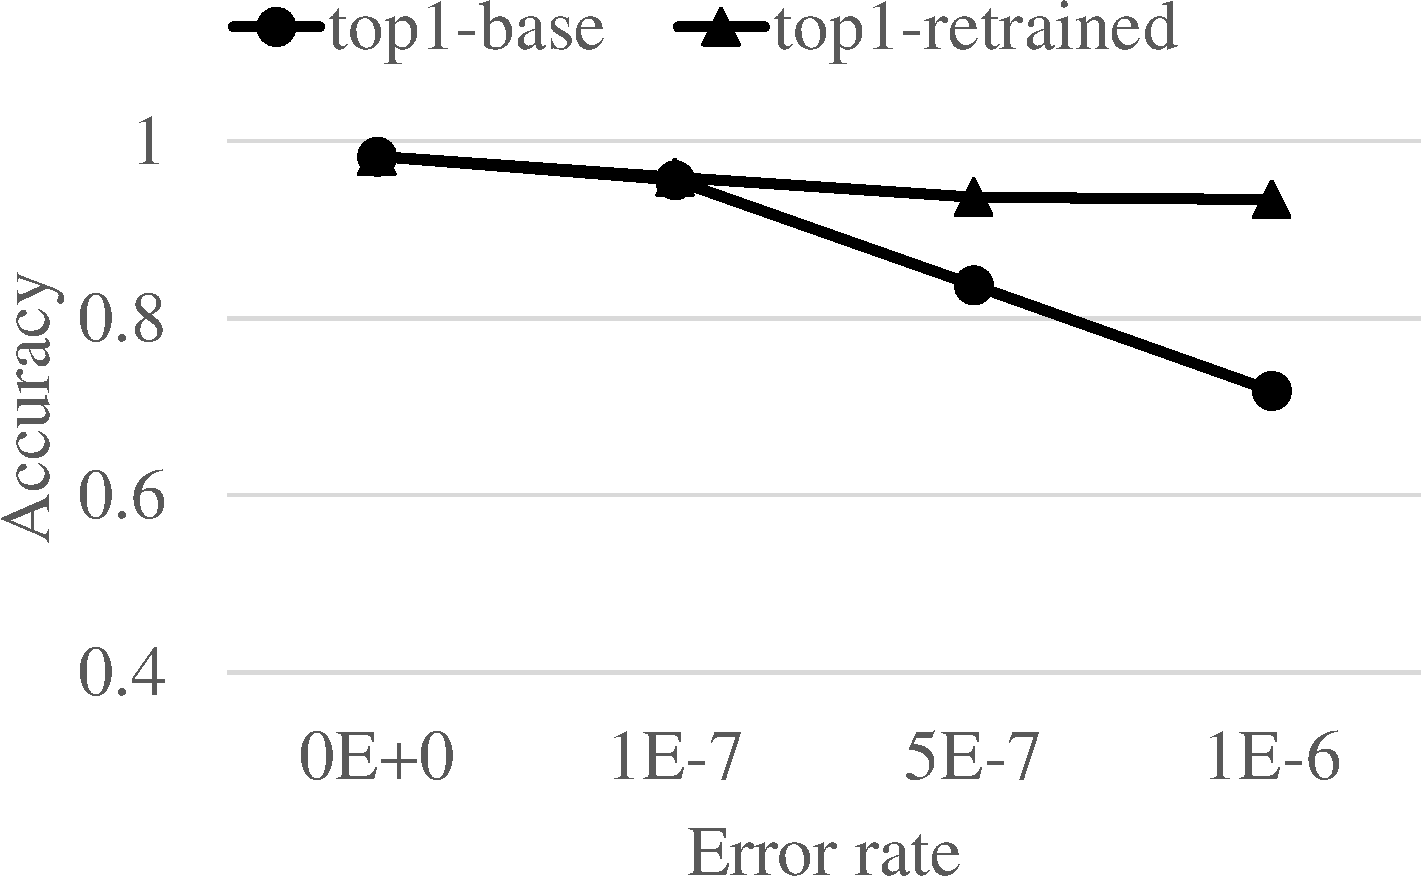
\includegraphics[width=0.6\linewidth]{lenet-softerror}
        }
        \qquad
        \subfloat[AlexNet]{
                \label{fig:alexnet}
                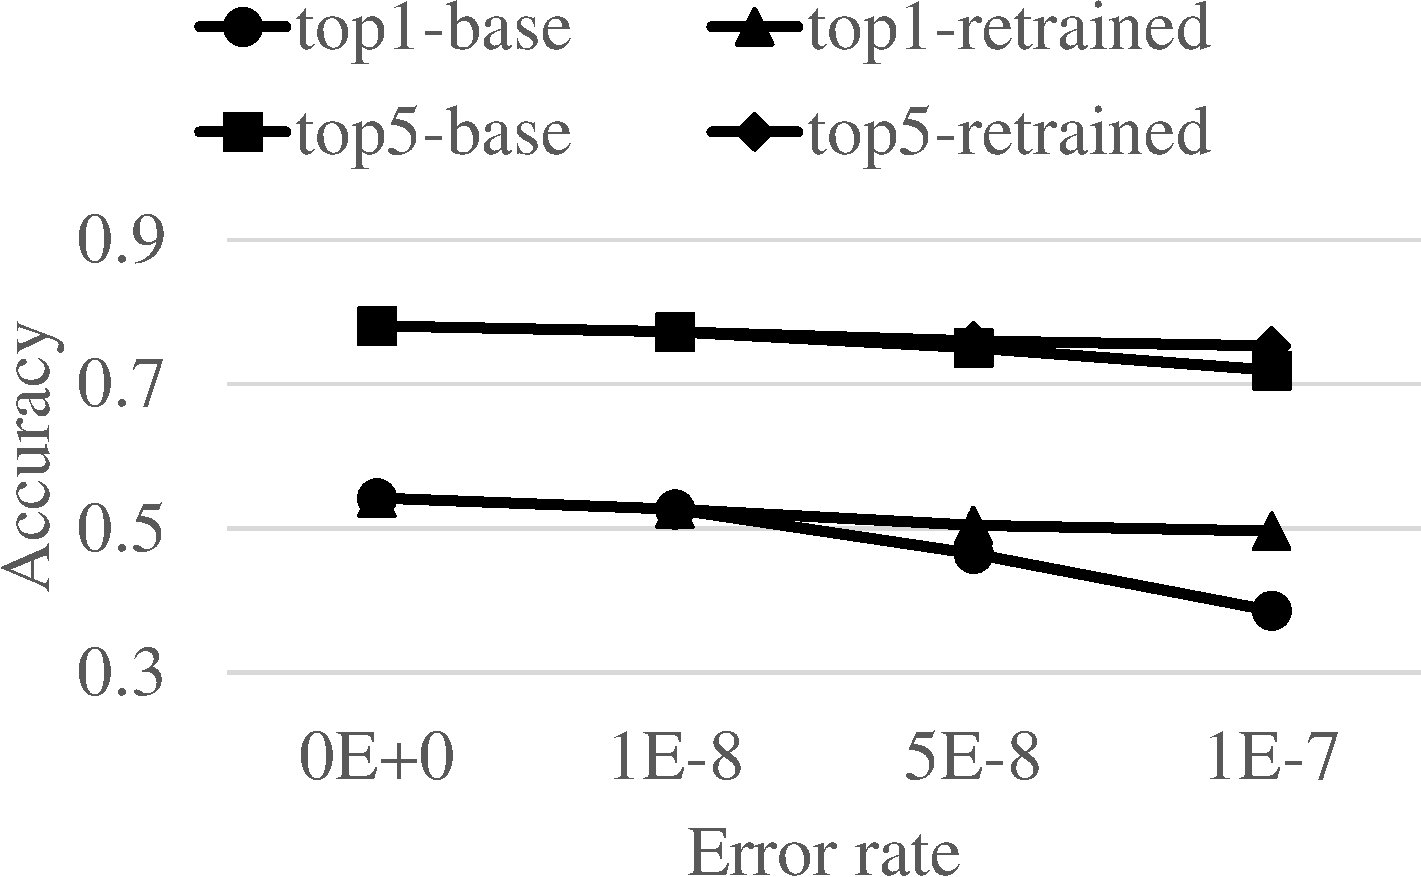
\includegraphics[width=0.6\linewidth]{alexnet-softerror}
        }
        \qquad
        \subfloat[VGG-16]{
                \label{fig:vgg16}
                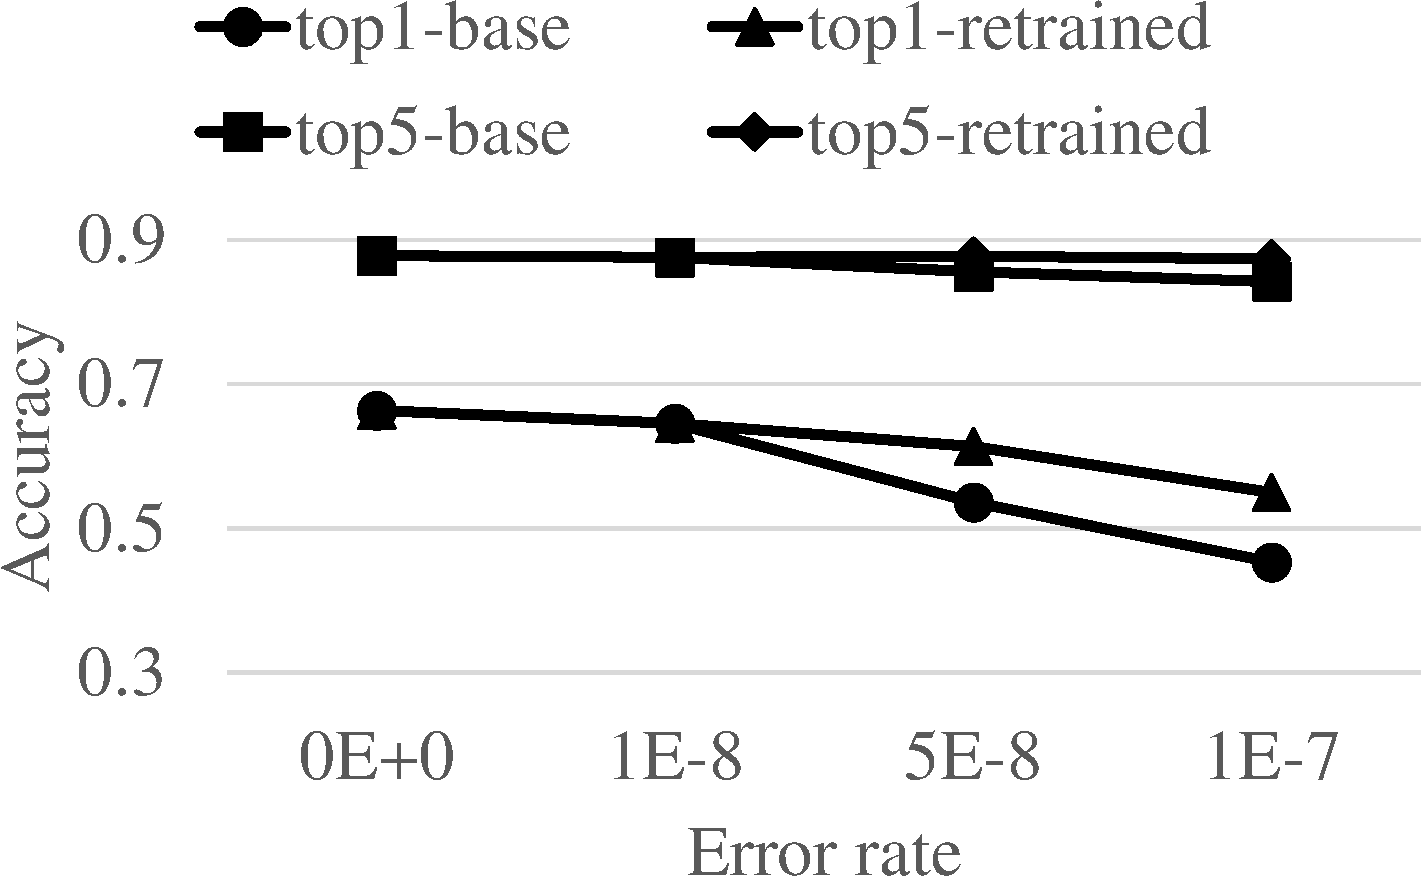
\includegraphics[width=0.6\linewidth]{vgg16-softerror}
        }
        \qquad
        \subfloat[VGG-19]{
                \label{fig:vgg19}
                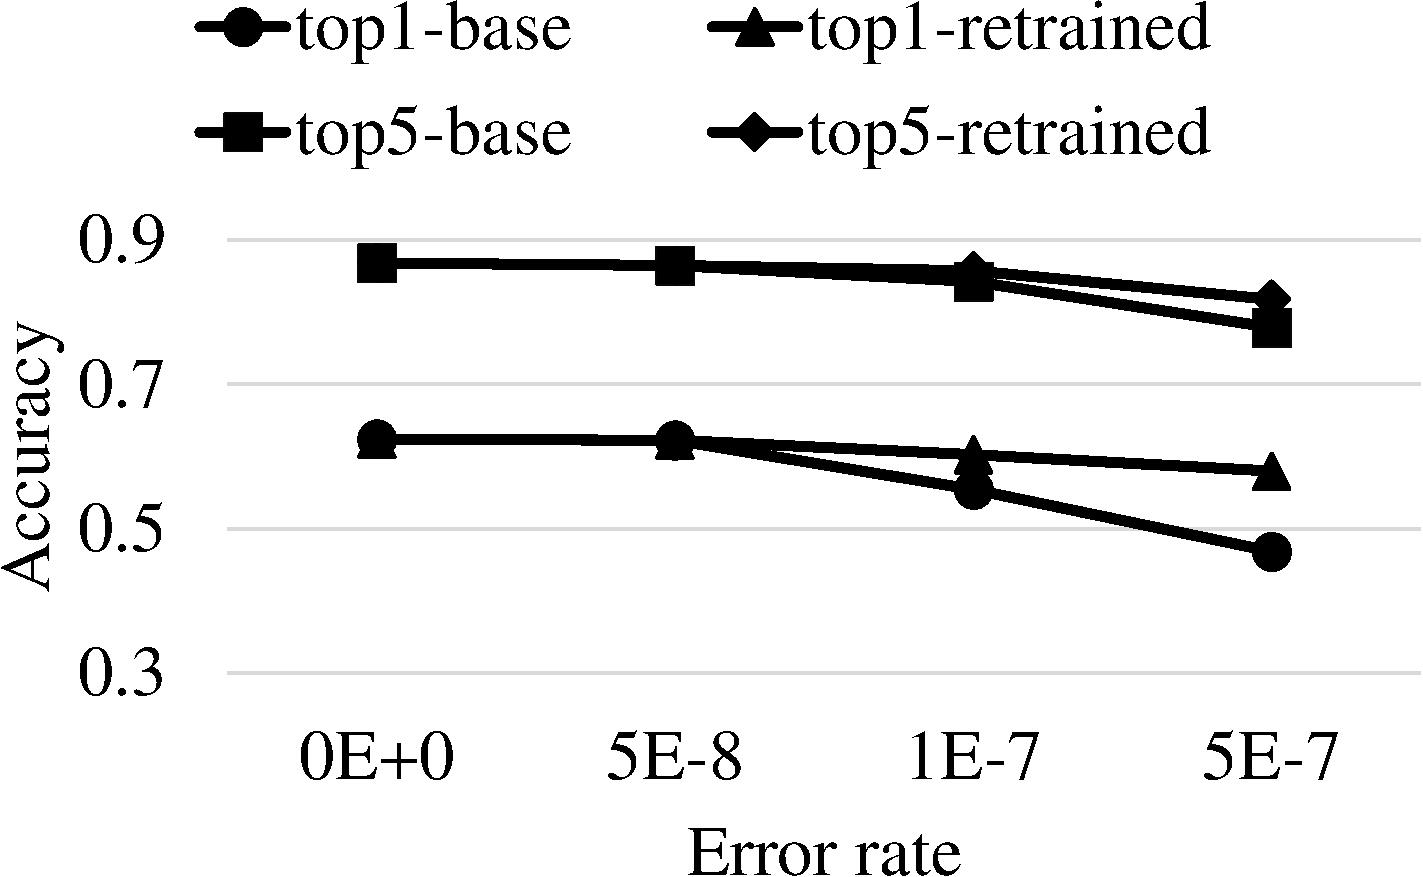
\includegraphics[width=0.6\linewidth]{vgg19-softerror}
        }
        \caption{The Precision of Four CNN models on accelerators with different error rate}
        \label{fig:softerror accuracy}
\end{figure}

  When the error injection rate goes higher, the proposed retraining becomes critical. 
According to the experiments, the accuracy of the four retrained models improve by 6.8\%, 1.5\%, 3\%, and 3\% 
respectively compared to that of the base model when the accelerators are exposed to the highest 
error injection. In summary, the experiments demonstrate that we can have the CNN model to learn 
both the characteristics of the data and the underlying ‘undeterministic’ behaviors of the accelerator 
together using the proposed training framework. The resulting CNN model can improve the accuracy 
without any modification on the accelerator when there is high error injection rate.  


